% ============================================================
%  يُترجَم بـ XeLaTeX  (في Overleaf: Menu → Compiler → XeLaTeX)
%  الخط: Amiri (متوفر في Overleaf، أو حمّله من github.com/aliftype/amiri)
% ============================================================
\documentclass[12pt,a4paper]{article}
\usepackage[a4paper,margin=1.7cm,top=2.3cm,bottom=2.9cm,headheight=15pt,footskip=1.5cm]{geometry}
\usepackage{amsmath,amssymb}
\usepackage{icomma}
\usepackage[english,bidi=default,layout=lists]{babel}
\babelprovide[import,main]{arabic}
\babelfont{rm}[Scale=1.08]{Amiri}
\babelfont{sf}[Scale=1.08]{Amiri}
\usepackage[most]{tcolorbox}
\usepackage{tikz}
\usetikzlibrary{arrows.meta,calc,shadings}
\usepackage{array}
\usepackage{colortbl}
\usepackage{fancyhdr}
\usepackage{titlesec}
\usepackage{enumitem}
\usepackage{collcell}
\usepackage{needspace}
\usepackage{etoolbox}
\newcolumntype{C}{>{\collectcell\ar}c<{\endcollectcell}}
\pretocmd{\section}{\Needspace{15\baselineskip}}{}{}
\pretocmd{\subsection}{\Needspace{11\baselineskip}}{}{}

\definecolor{cDef}{HTML}{1F4E9C}
\definecolor{cThm}{HTML}{B3261E}
\definecolor{cRem}{HTML}{2E7D32}
\definecolor{cEx}{HTML}{C76B00}
\definecolor{cMeth}{HTML}{6A1B9A}
\definecolor{cSol}{HTML}{00695C}
\definecolor{cSec}{HTML}{1F3A68}

\titleformat{\section}{\Large\bfseries\color{cSec}}{\thesection.}{0.6em}{}[{\color{cSec!60}\titlerule[1pt]}]
\titleformat{\subsection}{\large\bfseries\color{cThm!85!black}}{\thesubsection.}{0.5em}{}
\titlespacing*{\section}{0pt}{14pt}{8pt}
\titlespacing*{\subsection}{0pt}{10pt}{5pt}
\setlength{\parindent}{0pt}
\setlength{\parskip}{4pt}
\setlist{itemsep=2pt,topsep=3pt}

\newtcolorbox{arbox}[3][]{enhanced,
  colback=#2!5,colframe=#2!80!black,arc=2mm,boxrule=0.8pt,
  left=6pt,right=6pt,top=8pt,bottom=5pt,
  fonttitle=\bfseries,coltitle=white,
  title={\foreignlanguage{arabic}{#3}},
  attach boxed title to top right={xshift=-5mm,yshift=-3mm},
  boxed title style={colback=#2!80!black,arc=1.5mm,boxrule=0pt},
  before upper={\selectlanguage{arabic}},
  before skip=8pt,after skip=8pt,breakable,#1}
\newenvironment{BOX}[2]{\begin{otherlanguage}{english}\begin{arbox}{#1}{#2}}{\end{arbox}\end{otherlanguage}}
\newenvironment{tarif}[1][تعريف]{\begin{BOX}{cDef}{#1}}{\end{BOX}}
\newenvironment{khassia}[1][خاصية]{\begin{BOX}{cThm}{#1}}{\end{BOX}}
\newenvironment{molahada}[1][ملاحظة]{\begin{BOX}{cRem}{#1}}{\end{BOX}}
\newenvironment{mithal}[1][مثال]{\begin{BOX}{cEx}{#1}}{\end{BOX}}
\newenvironment{tariqa}[1][طريقة]{\begin{BOX}{cMeth}{#1}}{\end{BOX}}

\newcounter{exo}
\newenvironment{tamrin}[1]{\stepcounter{exo}\begin{BOX}{cSec}{التمرين \theexo: #1}}{\end{BOX}}
\newenvironment{hal}{\Needspace{12\baselineskip}\begin{otherlanguage}{english}\begin{arbox}[breakable]{cSol}{حل التمرين \theexo}}{\end{arbox}\end{otherlanguage}}

\newenvironment{LTR}{\begin{otherlanguage}{english}}{\end{otherlanguage}}
\newcommand{\ar}[1]{\foreignlanguage{arabic}{#1}}

\renewcommand{\dots}{\mathinner{\ldotp\ldotp\ldotp}}
\renewcommand{\ldots}{\mathinner{\ldotp\ldotp\ldotp}}
\renewcommand{\cdots}{\mathinner{\cdotp\cdotp\cdotp}}
\newcommand{\N}{\mathbb{N}}
\newcommand{\Z}{\mathbb{Z}}
\newcommand{\D}{\mathbb{D}}
\newcommand{\Q}{\mathbb{Q}}
\newcommand{\R}{\mathbb{R}}
\newcommand{\pgcd}{\operatorname{PGCD}}
\newcommand{\ppcm}{\operatorname{PPCM}}

% \NLseg{a}{b}{[}{]} ; \NLright{a}{[} ; \NLleft{b}{]}  (interval on a number line)
\newcommand{\NLseg}[4]{\begin{LTR}\begin{tikzpicture}[baseline=-0.6ex]
 \draw[-{Stealth[length=2mm]},gray!70](0,0)--(3.4,0);
 \draw[line width=2pt,cThm!80!black](0.7,0)--(2.7,0);
 \node[cThm!80!black,font=\LARGE] at (0.7,0){$#3$};
 \node[cThm!80!black,font=\LARGE] at (2.7,0){$#4$};
 \node[below=3pt,font=\footnotesize] at (0.7,0){$#1$};
 \node[below=3pt,font=\footnotesize] at (2.7,0){$#2$};
\end{tikzpicture}\end{LTR}}
\newcommand{\NLright}[2]{\begin{LTR}\begin{tikzpicture}[baseline=-0.6ex]
 \draw[-{Stealth[length=2mm]},gray!70](0,0)--(3.4,0);
 \draw[line width=2pt,cThm!80!black](1.3,0)--(3.3,0);
 \node[cThm!80!black,font=\LARGE] at (1.3,0){$#2$};
 \node[below=3pt,font=\footnotesize] at (1.3,0){$#1$};
\end{tikzpicture}\end{LTR}}
\newcommand{\NLleft}[2]{\begin{LTR}\begin{tikzpicture}[baseline=-0.6ex]
 \draw[-{Stealth[length=2mm]},gray!70](0,0)--(3.4,0);
 \draw[line width=2pt,cThm!80!black](0.05,0)--(2.1,0);
 \node[cThm!80!black,font=\LARGE] at (2.1,0){$#2$};
 \node[below=3pt,font=\footnotesize] at (2.1,0){$#1$};
\end{tikzpicture}\end{LTR}}

% ---------- social-media icons (pure TikZ) ----------
\definecolor{cFB}{HTML}{1877F2}
\definecolor{cTG}{HTML}{229ED9}
\definecolor{cIG1}{HTML}{FEDA75}
\definecolor{cIG2}{HTML}{D62976}
\definecolor{cIG3}{HTML}{4F5BD5}
\newcommand{\fbicon}{\begin{LTR}\begin{tikzpicture}[baseline=-0.75ex,x=1em,y=1em]
 \fill[cFB] (0,0) circle (0.55);
 \node[white,inner sep=0,font=\usefont{TU}{lmss}{bx}{n}\small] at (0.04,-0.02) {f};
\end{tikzpicture}\end{LTR}}
\newcommand{\igicon}{\begin{LTR}
\begin{tikzpicture}[baseline=-0.75ex,x=1em,y=1em]
 \shade[lower left=cIG1,lower right=cIG2,upper left=cIG2,upper right=cIG3,rounded corners=0.28em] (-0.55,-0.55) rectangle (0.55,0.55);
 \draw[white,line width=0.09em,rounded corners=0.18em] (-0.36,-0.36) rectangle (0.36,0.36);
 \draw[white,line width=0.09em] (0,0) circle (0.17);
 \fill[white] (0.22,0.22) circle (0.05);
\end{tikzpicture}\end{LTR}}
\newcommand{\tgicon}{\begin{LTR}
\begin{tikzpicture}[baseline=-0.75ex,x=1em,y=1em]
 \fill[cTG] (0,0) circle (0.55);
 \fill[white] (-0.33,0.0) -- (0.32,0.27) -- (0.2,-0.3) -- (0.0,-0.15) -- (-0.08,-0.28) -- (-0.08,-0.08) -- cycle;
 \fill[cTG!70!black] (-0.08,-0.08) -- (0.25,0.2) -- (0.0,-0.15) -- (-0.08,-0.28) -- cycle;
\end{tikzpicture}\end{LTR}}
% page number: black box, white two-digit number, at the right of the social row
\newcommand{\PageBox}{\begin{LTR}\tikz[baseline=(p.base)]\node[fill=black,text=white,inner sep=2.5pt,minimum width=1.6em,minimum height=1.3em,font=\usefont{TU}{lmss}{bx}{n}\small](p){\ifnum\value{page}<10 0\fi\arabic{page}};\end{LTR}}
% visual left-to-right order: Telegram | Instagram | Facebook | page box
\newcommand{\SocialRow}{\begin{otherlanguage}{english}%
 \ar{\textbf{الأستاذ سوايسية هشام للرياضيات}}\ \tgicon\hfill
 \textbf{prof\_hicham\_math}\ \igicon\hfill
 \ar{\textbf{الأستاذ سوايسية هشام للرياضيات}}\ \fbicon\hspace{2.2em}\PageBox\end{otherlanguage}}

\pagestyle{fancy}
\fancyhf{}
\renewcommand{\headrulewidth}{0.6pt}
\renewcommand{\footrulewidth}{0.4pt}
% \SetHeader{right head: document title}{left head: level -- stream}
\newcommand{\SetHeader}[2]{%
 \fancyhead[C]{\parbox{\textwidth}{\ar{#1\hfill #2}}}%
 \fancyfoot[C]{\parbox{\textwidth}{\small\SocialRow}}}
\usepackage{tkz-tab}
\usepackage{multicol}
% variation / sign table (LTR)
\newenvironment{TAB}{\par\begin{center}\begin{LTR}\begin{tikzpicture}[scale=0.95,every node/.style={font=\small}]}{\end{tikzpicture}\end{LTR}\end{center}}
% grid + axes, clipped: \begin{GR}{xmin}{xmax}{ymin}{ymax}{unit cm}
\newenvironment{GR}[5]{\par\begin{center}\begin{LTR}\begin{tikzpicture}[x=#5cm,y=#5cm,font=\footnotesize]
 \draw[gray!25,very thin] (#1,#3) grid (#2,#4);
 \draw[-{Stealth[length=2mm]}] (#1,0)--(#2+0.3,0) node[below left]{$x$};
 \draw[-{Stealth[length=2mm]}] (0,#3)--(0,#4+0.3) node[below left]{$y$};
 \node[below left] at (0,0){$O$};
 \begin{scope}\clip (#1,#3) rectangle (#2,#4);}
{\end{scope}\end{tikzpicture}\end{LTR}\end{center}}
\newcommand{\Ticks}[2]{\foreach \t in {#1} \node[below,font=\scriptsize] at (\t,0){$\t$}; \foreach \t in {#2} \node[left,font=\scriptsize] at (0,\t){$\t$};}
\newcommand{\bx}[1]{\ensuremath{\colorbox{cDef!12}{$\displaystyle #1$}}}
\newcommand{\TwoCol}[4]{\par\begin{LTR}\noindent\begin{minipage}[t]{#1\textwidth}\selectlanguage{arabic}#2\end{minipage}\hfill\begin{minipage}[t]{#3\textwidth}\selectlanguage{arabic}#4\end{minipage}\end{LTR}\par}
\newcommand{\RL}[4]{\TwoCol{#3}{#4}{#1}{#2}}  % \RL{w1}{right content}{w2}{left content}
\newcommand{\ok}{$\textcolor{cRem}{\checkmark}$}
\newcommand{\limn}{\displaystyle\lim_{n\to+\infty}}
% sub-questions, each on its own line
\newenvironment{sq}{\begin{itemize}[leftmargin=2.4em,itemsep=3pt]}{\end{itemize}}
\newcommand{\qa}{\item[(أ)]}\newcommand{\qb}{\item[(ب)]}\newcommand{\qc}{\item[(جـ)]}\newcommand{\qd}{\item[(د)]}\newcommand{\qe}{\item[(هـ)]}
\newcommand{\pa}{\par\smallskip\textbf{(أ)} }\newcommand{\pb}{\par\smallskip\textbf{(ب)} }\newcommand{\pc}{\par\smallskip\textbf{(جـ)} }\newcommand{\pd}{\par\smallskip\textbf{(د)} }\newcommand{\pe}{\par\smallskip\textbf{(هـ)} }
\newcommand{\QQ}[1]{\par\smallskip\textbf{#1.} }
\newenvironment{tmr}{\stepcounter{exo}\begin{BOX}{cSec}{تمرين محلول \theexo}}{\end{BOX}}
\newcommand{\ABC}[3]{\\[2pt]\begin{tabular}{p{0.28\textwidth}p{0.28\textwidth}p{0.28\textwidth}}(جـ) \ #3 & (ب) \ #2 & (أ) \ #1\end{tabular}}
\pretocmd{\section}{\Needspace{24\baselineskip}}{}{}
\newtcbox{\bxtbox}{on line,colback=cDef!12,colframe=cDef!12,boxrule=0pt,arc=1pt,boxsep=0pt,left=2pt,right=2pt,top=1pt,bottom=1pt}
\newcommand{\bxt}[1]{\foreignlanguage{english}{\bxtbox{\ar{#1}}}}
\usepackage{longtable}
\setlength{\LTpre}{4pt}\setlength{\LTpost}{0pt}
\newcommand{\Phase}[1]{\textbf{#1}}
\newcommand{\Fld}[2]{\textbf{#1:}\ #2}
% رأس المذكرة على نمط النموذج: إطار بعنوان «مذكرة رقم»، معلومات الحصة، ثم إطار الكفاءات
\newcommand{\ModhHead}[9]{%
\begin{LTR}
\begin{tcolorbox}[enhanced,colback=white,colframe=cThm!85!black,arc=4mm,boxrule=1pt,top=14pt,bottom=6pt,left=8pt,right=8pt,
 overlay={\node[fill=cThm!85!black,text=white,rounded corners=3mm,inner xsep=14pt,inner ysep=4pt,font=\large\bfseries] at ([yshift=0pt]frame.north){\ar{مذكرة رقم #1}};},
 before upper={\selectlanguage{arabic}}]
\begin{tabular}{@{}p{0.4\linewidth}p{0.55\linewidth}@{}}
\Fld{المستوى}{#2} & \Fld{الثانوية}{\dotfill}\\[3pt]
\Fld{المادة}{رياضيات} & \Fld{ميدان التعلم}{#3}\\[3pt]
\Fld{المدة}{#5} & \Fld{الوحدة التعلمية}{#4}\\[3pt]
\Fld{الأستاذ}{\dotfill} & \Fld{المحتوى المعرفي}{#6}\\
\end{tabular}
\end{tcolorbox}
\begin{tcolorbox}[enhanced,colback=white,colframe=cThm!85!black,arc=3mm,boxrule=0.8pt,sidebyside,sidebyside align=top,lefthand ratio=0.5,
 segmentation style={dashed,cThm!60},before upper={\selectlanguage{arabic}},before lower={\selectlanguage{arabic}}]
\textbf{الكفاءات المستهدفة:}\par #8
\tcblower
\textbf{الكفاءات القبلية:}\par #7
\end{tcolorbox}
\end{LTR}
\par\smallskip\textbf{الوسائل:} #9\par\smallskip}
\newenvironment{Sayr}{%
\begin{LTR}\renewcommand{\arraystretch}{1.25}
\begin{longtable}{|p{0.17\textwidth}|>{\centering\arraybackslash}p{0.06\textwidth}|p{0.53\textwidth}|>{\centering\arraybackslash}p{0.12\textwidth}|}
\hline\rowcolor{cThm!12}\ar{\textbf{توجيهات وتعاليق}} & \ar{\textbf{المدة}} & \ar{\textbf{سير الحصة}} & \ar{\textbf{مراحل الحصة}}\\\hline\endhead
\hline\endfoot}{\end{longtable}\end{LTR}}
% سطر في الجدول: \Row{مرحلة}{سير}{مدة}{توجيهات}
\newcommand{\Row}[4]{\ar{\small #4} & \ar{#3} & \ar{#2} & \cellcolor{cThm!8}\ar{\Phase{#1}}\\\hline}

\newcommand{\Lab}[2]{\foreignlanguage{english}{\tcbox[on line,colback=#1,colframe=#1,boxrule=0pt,arc=2pt,boxsep=1pt,left=5pt,right=5pt,top=1pt,bottom=1pt]{\ar{\textcolor{white}{\textbf{#2}}}}}}
\newcommand{\Num}[1]{\foreignlanguage{english}{\tikz[baseline=(c.base)]\node[fill=cDef,text=white,inner sep=2pt,font=\footnotesize\bfseries](c){#1};}}
\newcommand{\ck}{\ensuremath{{\color{cRem}\checkmark}}}
\newenvironment{Kad}[1]{\par\smallskip\Lab{#1}}{\par}
\SetHeader{\small\bfseries\color{cSec}مذكرات محور: الهندسة في الفضاء}{\small\color{cSec}السنة الثانية ثانوي -- علوم تجريبية}
\begin{document}
\begin{LTR}
\begin{tcolorbox}[enhanced,colback=cThm!85!black,colframe=cThm!85!black,arc=3mm,halign=center,boxrule=0pt,top=12pt,bottom=12pt,before upper={\selectlanguage{arabic}}]
{\color{white}\fontsize{26}{32}\selectfont\bfseries مذكرات محور: الهندسة في الفضاء}\\[8pt]
{\color{white}\large السنة الثانية ثانوي -- علوم تجريبية (صالحة لشعبتي رياضيات وتقني رياضي)}\\[4pt]
{\color{white}\large 8 مذكرات (16 ساعة) -- السنة الدراسية 2026-2027}
\end{tcolorbox}
\end{LTR}
\begin{BOX}{cThm}{يتضمن هذا العمل}
\begin{enumerate}[label=\textbf{مذكرة \arabic{enumi}:},leftmargin=6em,start=64]
\item المجسمات: التمثيل والأطوال والمساحات والحجوم.
\item الأوضاع النسبية لمستقيمات ومستويات.
\item التوازي والتعامد في الفضاء.
\item المقاطع المستوية (رياضيات وتقني رياضي).
\item الحساب الشعاعي في الفضاء.
\item المعلم في الفضاء: الإحداثيات ، المسافة ، مستو مواز لمستوي إحداثيات.
\item التمثيل الوسيطي لمستقيم في الفضاء.
\item معادلة سطح كرة.
\end{enumerate}
مراجع النشاطات: الكتاب المدرسي للسنة الثانية ثانوي (باب المقاطع المستوية والأشعة في الفضاء ص 270--271 ، باب التعليم في الفضاء). شعبة العلوم التجريبية: لا مقاطع مستوية ، وسطح الكرة فقط.
\end{BOX}
\newpage
\ModhHead{64}{2 ع ت}{هندسة}{الهندسة في الفضاء}{02 سا}{المجسمات: التمثيل والأطوال والمساحات والحجوم}%
{\begin{itemize}\item الهندسة في الفضاء (1 ج م) ، مبرهنة فيثاغورس.\end{itemize}}%
{\begin{itemize}\item تمثيل مجسم بالمنظور متساوي القياس وإنشاء تصميمه.\item حساب أطوال ومساحات وحجوم المجسمات المألوفة.\end{itemize}}%
{المنهاج ، الكتاب المدرسي ، مراجع ، مجسمات ، برنامج GeoGebra.}
\begin{Sayr}
\Row{مرحلة الانطلاق}{%
\textbf{التهيئة النفسية:} كيف نرسم مكعباً على ورقة مستوية؟ وما الذي لا يُحفظ في الرسم؟}{10 د}{مجسمات حقيقية في القسم.}
\Row{التشخيص والاكتشاف}{%
\Lab{cEx}{وضعية مقترحة}\ مكعب $ABCDEFGH$ حرفه $3$ cm.\par\ck\ نرسمه بالمنظور متساوي القياس: الأحرف المخفية بالمتقطع ، والمتوازية تبقى متوازية.\par
\ck\ نحسب طول القطر $[AG]$ بتطبيق فيثاغورس مرتين: $AC=3\sqrt2$ ، $AG=3\sqrt3$.\par
}{35 د}{رسم بالمنظور.}
\Row{بناء المعارف}{%
\Lab{cThm}{المنظور متساوي القياس}\ يحافظ على التوازي ومنتصفات القطع ونسب الأطوال على مستقيم واحد ، ولا يحافظ على الزوايا ولا على كل الأطوال.\par\smallskip\begin{LTR}\centering 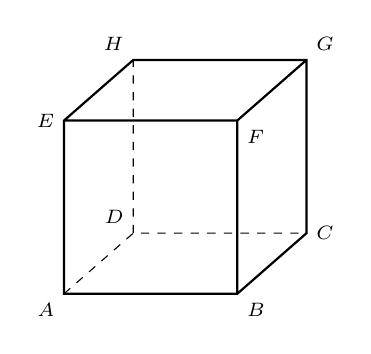
\begin{tikzpicture}[scale=1.1,font=\scriptsize]
\coordinate (A) at (0,0); \coordinate (B) at (2,0); \coordinate (C) at (2.8,0.7); \coordinate (D) at (0.8,0.7);
\coordinate (E) at (0,2); \coordinate (F) at (2,2); \coordinate (G) at (2.8,2.7); \coordinate (H) at (0.8,2.7);
\draw[thick] (A)--(B)--(C)--(G)--(H)--(E)--cycle (B)--(F)--(E) (F)--(G);
\draw[dashed] (A)--(D)--(C) (D)--(H);
\foreach \p/\q in {A/below left,B/below right,C/right,D/above left,E/left,F/below right,G/above right,H/above left} \node[\q] at (\p){$\p$};
\end{tikzpicture}\end{LTR}\par \Lab{cThm}{الحجوم}\par\ck\ متوازي مستطيلات: $V=abc$ ؛ موشور وأسطوانة: $V=B\times h$.\par
\ck\ هرم: $V=\frac13B\times h$ ؛ كرة: $V=\frac43\pi r^3$ ومساحتها $4\pi r^2$.\par
}{50 د}{جدول الحجوم يُحفظ.}
\Row{}{%
\Lab{cEx}{مثال}\ هرم قاعدته مربع ضلعه $4$ وارتفاعه $6$: $V=\frac13\times16\times6=32$ ؛ أسطوانة $r=2$ ، $h=5$: $V=20\pi$.\par\Lab{cThm!80!black}{حذار}\ في الرسم بالمنظور لا نقيس الأطوال مباشرة.}{}{}
\Row{التقويم}{%
\Lab{cEx}{تطبيق}\par متوازي مستطيلات أبعاده $2$ ، $3$ ، $6$. احسب حجمه وطول قطره ، ثم حجم كرة نصف قطرها $3$.\par\textbf{الحل:} $V=36$ ؛ القطر $\sqrt{4+9+36}=7$ ؛ $V=\frac43\pi\times27=36\pi$.\par\textbf{واجب منزلي:} تمارين من الكتاب المدرسي.\par\smallskip\textbf{ملاحظات حول سير الحصة:} \dotfill}{25 د}{تقويم فردي.}
\end{Sayr}
\newpage
\ModhHead{65}{2 ع ت}{هندسة}{الهندسة في الفضاء}{02 سا}{الأوضاع النسبية لمستقيمات ومستويات}%
{\begin{itemize}\item المجسمات وتمثيلها.\end{itemize}}%
{\begin{itemize}\item تعيين الوضع النسبي لمستقيمين ، لمستقيم ومستو ، ولمستويين.\end{itemize}}%
{المنهاج ، الكتاب المدرسي ، مراجع ، مجسمات ، برنامج GeoGebra.}
\begin{Sayr}
\Row{مرحلة الانطلاق}{%
\textbf{التهيئة النفسية:} في القسم: حافتا السقف والأرض المتقابلتان ، هل تتقاطعان؟ هل هما متوازيتان؟}{10 د}{أمثلة من القسم.}
\Row{التشخيص والاكتشاف}{%
\Lab{cEx}{وضعية مقترحة}\ في المكعب $ABCDEFGH$: ما الوضع النسبي لـ $(AB)$ و $(HG)$ ؟ $(AB)$ و $(CG)$ ؟ $(AE)$ والمستوي $(ABC)$ ؟\par\ck\ $(AB)\parallel(HG)$ ؛ $(AB)$ و $(CG)$ \textbf{ليسا من نفس المستوي} (لا يتقاطعان ولا يتوازيان).\par
}{35 د}{مكعب حقيقي.}
\Row{بناء المعارف}{%
\Lab{cThm}{مستقيمان}\ إما من نفس المستوي (متقاطعان أو متوازيان) ، وإما ليسا من نفس المستوي.\par\Lab{cThm}{مستقيم ومستو}\ المستقيم محتوى في المستوي ، أو يقطعه في نقطة ، أو يوازيه تماماً.\par}{50 د}{جدول الحالات.}
\Row{}{%
\Lab{cThm}{مستويان}\ متقاطعان وفق مستقيم ، أو متوازيان (تماماً أو منطبقان).\par\Lab{cEx}{مثال}\ $(AE)$ يقطع $(ABC)$ في $A$ ؛ $(ABC)\parallel(EFG)$ ؛ $(ABF)$ و $(BCG)$ يتقاطعان وفق $(BF)$.\par}{}{}
\Row{}{%
\Lab{cThm!80!black}{حذار}\ مستقيمان لا يتقاطعان ليسا بالضرورة متوازيين في الفضاء.}{}{}
\Row{التقويم}{%
\Lab{cEx}{تطبيق}\par في المكعب: عيّن الوضع النسبي لـ: $(EG)$ و $(AC)$ ؛ $(BH)$ و $(ADE)$ ؛ $(ACG)$ و $(BDF)$.\par\textbf{الحل:} متوازيان ؛ متقاطعان في $H$ ؛ متقاطعان وفق المستقيم الذي يشمل مركزي الوجهين $ABCD$ و $EFGH$.\par\textbf{واجب منزلي:} تمارين من الكتاب المدرسي.\par\smallskip\textbf{ملاحظات حول سير الحصة:} \dotfill}{25 د}{تقويم فردي.}
\end{Sayr}
\newpage
\ModhHead{66}{2 ع ت}{هندسة}{الهندسة في الفضاء}{02 سا}{التوازي والتعامد في الفضاء}%
{\begin{itemize}\item الأوضاع النسبية.\end{itemize}}%
{\begin{itemize}\item استعمال خواص التوازي والتعامد في الفضاء.\end{itemize}}%
{المنهاج ، الكتاب المدرسي ، مراجع ، مجسمات ، برنامج GeoGebra.}
\begin{Sayr}
\Row{مرحلة الانطلاق}{%
\textbf{التهيئة النفسية:} كيف يتأكد البنّاء أن العمود عمودي على الأرض؟ هل يكفي قياس زاوية واحدة؟}{10 د}{سؤال من الحياة.}
\Row{التشخيص والاكتشاف}{%
\Lab{cEx}{وضعية مقترحة}\ في المكعب: $(AE)\perp(AB)$ و $(AE)\perp(AD)$.\par\ck\ نستنتج أن $(AE)$ عمودي على كل مستقيم من المستوي $(ABD)$.\par
}{35 د}{مكعب حقيقي.}
\Row{بناء المعارف}{%
\Lab{cThm}{التوازي}\par\ck\ إذا وازى مستقيم مستقيماً من مستو فهو يوازي هذا المستوي.\par
\ck\ إذا وازى مستقيمان متقاطعان من مستو مستوياً آخر فالمستويان متوازيان.\par
\ck\ إذا قطع مستو مستويين متوازيين فالمستقيمان الناتجان متوازيان.\par
\Lab{cThm}{التعامد}\par\ck\ مستقيم عمودي على مستو إذا كان عمودياً على مستقيمين متقاطعين منه.\par
\ck\ إذا كان مستقيم عمودياً على مستو فهو عمودي على كل مستقيم منه.\par
}{50 د}{نلون المستوي والمستقيم.}
\Row{}{%
\Lab{cEx}{مثال}\ $(BD)\perp(AC)$ و $(BD)\perp(AE)$ ، إذن $(BD)\perp(ACE)$ ، ومنه $(BD)\perp(AG)$.\par\Lab{cThm!80!black}{حذار}\ التعامد مع مستقيم واحد من المستوي لا يكفي.}{}{}
\Row{التقويم}{%
\Lab{cEx}{تطبيق}\par في المكعب: بيّن أن $(EG)\parallel(ABC)$ ، وأن $(FB)\perp(ABC)$.\par\textbf{الحل:} $(EG)\parallel(AC)$ و $(AC)\subset(ABC)$ ؛ $(FB)\perp(AB)$ و $(FB)\perp(BC)$.\par\textbf{واجب منزلي:} تمارين من الكتاب المدرسي.\par\smallskip\textbf{ملاحظات حول سير الحصة:} \dotfill}{25 د}{تقويم فردي.}
\end{Sayr}
\newpage
\ModhHead{67}{2 ع ت}{هندسة}{الهندسة في الفضاء}{02 سا}{المقاطع المستوية: مقطع مكعب ورباعي وجوه بمستو (رياضيات وتقني رياضي)}%
{\begin{itemize}\item التوازي في الفضاء.\end{itemize}}%
{\begin{itemize}\item إنشاء مقطع مكعب أو رباعي وجوه بمستو.\end{itemize}}%
{المنهاج ، الكتاب المدرسي ، مراجع ، مجسمات ، برنامج GeoGebra.}
\begin{Sayr}
\Row{مرحلة الانطلاق}{%
\textbf{التهيئة النفسية:} نقطع قطعة جبن مكعبة بسكين مستقيمة: ما أشكال المقطع الممكنة؟}{10 د}{تجربة بجسم حقيقي.}
\Row{التشخيص والاكتشاف}{%
\Lab{cEx}{مناقشة النشاطين 01 و 02 صفحة 270}\par\ck\ تقاطع مستو مع أوجه المكعب: قطع مستقيمة نصلها.\par
\ck\ تقاطع مستو مع رباعي وجوه: مستقيم تقاطع مستويين.\par
}{35 د}{نشاطا الكتاب.}
\Row{بناء المعارف}{%
\Lab{cMeth}{طريقة}\par\ck\ نبحث عن نقطتين مشتركتين بين المستوي ووجه: نصلهما.\par
\ck\ إذا قطع المستوي وجهين متوازيين فالقطعتان متوازيتان.\par
\ck\ نمدد الأحرف لإيجاد نقط تقاطع مساعدة إذا لزم.\par
\Lab{cEx}{مقطع مكعب بمستو يمر بمنتصفات ثلاثة أحرف}\par\smallskip\begin{LTR}\centering 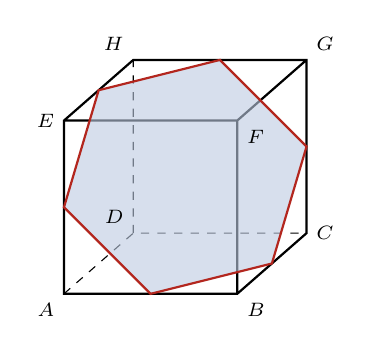
\begin{tikzpicture}[scale=1.1,font=\scriptsize]
\coordinate (A) at (0,0); \coordinate (B) at (2,0); \coordinate (C) at (2.8,0.7); \coordinate (D) at (0.8,0.7);
\coordinate (E) at (0,2); \coordinate (F) at (2,2); \coordinate (G) at (2.8,2.7); \coordinate (H) at (0.8,2.7);
\coordinate (I) at (1,0); \coordinate (J) at (2.4,0.35); \coordinate (K) at (2.8,1.7);
\draw[thick] (A)--(B)--(C)--(G)--(H)--(E)--cycle (B)--(F)--(E) (F)--(G);
\draw[dashed] (A)--(D)--(C) (D)--(H);
\fill[cDef!30,opacity=0.6] (I)--(J)--(K)--(1.8,2.7)--(0.4,2.35)--(0,1.0)--cycle;
\draw[cThm,thick] (I)--(J)--(K)--(1.8,2.7)--(0.4,2.35)--(0,1.0)--cycle;
\foreach \p/\q in {A/below left,B/below right,C/right,D/above left,E/left,F/below right,G/above right,H/above left} \node[\q] at (\p){$\p$};
\end{tikzpicture}\end{LTR}\par المقطع سداسي منتظم.\par}{50 د}{GeoGebra 3D.}
\Row{}{%
\Lab{cThm!80!black}{حذار}\ المقطع يتكون من قطع على \textbf{الأوجه} فقط.}{}{}
\Row{التقويم}{%
\Lab{cEx}{تطبيق}\par $ABCD$ رباعي وجوه ، $I$ و $J$ منتصفا $[AB]$ و $[AC]$ ، $K$ نقطة من $[AD]$. أنشئ مقطع رباعي الوجوه بالمستوي $(IJK)$.\par\textbf{الحل:} المقطع هو المثلث $IJK$ (القطع $[IJ]$ ، $[JK]$ ، $[KI]$ على الأوجه $ABC$ ، $ACD$ ، $ABD$).\par\textbf{واجب منزلي:} تمارين من باب المقاطع المستوية.\par\smallskip\textbf{ملاحظات حول سير الحصة:} \dotfill}{25 د}{شعبة العلوم التجريبية: حصة دعم بدلها.}
\end{Sayr}
\newpage
\ModhHead{68}{2 ع ت}{هندسة}{الهندسة في الفضاء}{02 سا}{الحساب الشعاعي في الفضاء}%
{\begin{itemize}\item الأشعة في المستوي ، علاقة شال.\end{itemize}}%
{\begin{itemize}\item إثبات توازي شعاعين واستقامية ثلاث نقط.\item إثبات أن أشعة من نفس المستوي.\end{itemize}}%
{المنهاج ، الكتاب المدرسي ، مراجع ، مجسمات ، برنامج GeoGebra.}
\begin{Sayr}
\Row{مرحلة الانطلاق}{%
\textbf{التهيئة النفسية:} هل تبقى علاقة شال صحيحة في الفضاء؟}{10 د}{سؤال.}
\Row{التشخيص والاكتشاف}{%
\Lab{cEx}{مناقشة النشاطين 03 و 05 صفحة 271}\par\ck\ نعبر عن شعاع بدلالة شعاعين آخرين بعلاقة شال.\par
\ck\ نستنتج توازي مستقيمين أو انتماء أشعة إلى نفس المستوي.\par
}{35 د}{نشاطا الكتاب.}
\Row{بناء المعارف}{%
\Lab{cThm}{خاصية}\par\ck\ قواعد الحساب الشعاعي في المستوي تبقى صحيحة في الفضاء.\par
\ck\ $\overrightarrow{AB}$ و $\overrightarrow{AC}$ مرتبطان خطياً إذا وفقط إذا كانت $A$ ، $B$ ، $C$ على استقامة واحدة.\par
\Lab{cDef}{أشعة من نفس المستوي}\ $\vec w$ و $\vec u$ و $\vec v$ ($\vec u$ ، $\vec v$ غير مرتبطين خطياً) من نفس المستوي إذا وُجد $a$ و $b$ حيث $\vec w=a\vec u+b\vec v$.\par}{50 د}{رسم الأشعة بالألوان.}
\Row{}{%
\Lab{cEx}{مثال}\ $ABCD$ رباعي وجوه ، $I$ و $J$ منتصفا $[AB]$ و $[CD]$: $\overrightarrow{IJ}=\overrightarrow{IA}+\overrightarrow{AD}+\overrightarrow{DJ}$ و $\overrightarrow{IJ}=\overrightarrow{IB}+\overrightarrow{BC}+\overrightarrow{CJ}$ ؛ بالجمع: $\overrightarrow{IJ}=\frac12(\overrightarrow{AD}+\overrightarrow{BC})$ ، إذن الأشعة $\overrightarrow{IJ}$ ، $\overrightarrow{AD}$ ، $\overrightarrow{BC}$ من نفس المستوي.\par\Lab{cThm!80!black}{حذار}\ أشعة من نفس المستوي لا تعني أن النقط من نفس المستوي.}{}{}
\Row{التقويم}{%
\Lab{cEx}{تطبيق}\par في المكعب $ABCDEFGH$: بيّن أن $\overrightarrow{AG}=\overrightarrow{AB}+\overrightarrow{AD}+\overrightarrow{AE}$.\par\textbf{الحل:} $\overrightarrow{AG}=\overrightarrow{AC}+\overrightarrow{CG}=(\overrightarrow{AB}+\overrightarrow{AD})+\overrightarrow{AE}$.\par\textbf{واجب منزلي:} تمارين من باب الأشعة في الفضاء.\par\smallskip\textbf{ملاحظات حول سير الحصة:} \dotfill}{25 د}{تقويم فردي.}
\end{Sayr}
\newpage
\ModhHead{69}{2 ع ت}{هندسة}{الهندسة في الفضاء}{02 سا}{المعلم في الفضاء: الإحداثيات ، المسافة ، مستو مواز لمستوي إحداثيات}%
{\begin{itemize}\item المعلم في المستوي ، الحساب الشعاعي في الفضاء.\end{itemize}}%
{\begin{itemize}\item تعليم نقط ، حساب مسافة ومنتصف.\item تعيين معادلة مستو مواز لأحد مستويات الإحداثيات.\end{itemize}}%
{المنهاج ، الكتاب المدرسي ، مراجع ، مجسمات ، برنامج GeoGebra.}
\begin{Sayr}
\Row{مرحلة الانطلاق}{%
\textbf{التهيئة النفسية:} كيف نحدد موقع طائرة في السماء؟ (خط العرض ، خط الطول ، الارتفاع)}{10 د}{سؤال من الحياة.}
\Row{التشخيص والاكتشاف}{%
\Lab{cEx}{مناقشة النشاطين 01 و 03 (أنشطة باب التعليم في الفضاء)}\par\ck\ إحداثيات رؤوس متوازي مستطيلات في معلم.\par
\ck\ حساب المسافة بتطبيق فيثاغورس في مثلثين قائمين.\par
}{35 د}{نشاطا الكتاب.}
\Row{بناء المعارف}{%
\Lab{cThm}{خاصية}\ في معلم متعامد ومتجانس $(O;\vec i,\vec j,\vec k)$:\par\ck\ $\overrightarrow{AB}(x_B-x_A;y_B-y_A;z_B-z_A)$ ؛ المنتصف $\left(\frac{x_A+x_B}2;\frac{y_A+y_B}2;\frac{z_A+z_B}2\right)$.\par
\ck\ $AB=\sqrt{(x_B-x_A)^2+(y_B-y_A)^2+(z_B-z_A)^2}$.\par
\ck\ المستوي الذي يشمل $A$ ويوازي $(xOy)$ معادلته $z=z_A$ (وبالمثل $x=x_A$ ، $y=y_A$).\par
\Lab{cEx}{مثال}\ $A(1;2;-1)$ ، $B(3;-2;3)$: $AB=\sqrt{4+16+16}=6$ ، المنتصف $(2;0;1)$ ؛ المستوي الذي يشمل $A$ ويوازي $(xOy)$: $z=-1$.\par}{50 د}{رسم المعلم بالمنظور.}
\Row{}{%
\Lab{cThm!80!black}{حذار}\ $z=-1$ في الفضاء مستوٍ وليس مستقيماً.}{}{}
\Row{التقويم}{%
\Lab{cEx}{تطبيق}\par $A(2;0;1)$ ، $B(0;2;1)$ ، $C(1;1;5)$. بيّن أن المثلث $ABC$ متساوي الساقين.\par\textbf{الحل:} $CA=\sqrt{1+1+16}=\sqrt{18}$ ، $CB=\sqrt{1+1+16}=\sqrt{18}$ ، $AB=\sqrt8$: متساوي الساقين رأسه $C$.\par\textbf{واجب منزلي:} تمارين من باب التعليم في الفضاء.\par\smallskip\textbf{ملاحظات حول سير الحصة:} \dotfill}{25 د}{تقويم فردي.}
\end{Sayr}
\newpage
\ModhHead{70}{2 ع ت}{هندسة}{الهندسة في الفضاء}{02 سا}{التمثيل الوسيطي لمستقيم في الفضاء}%
{\begin{itemize}\item الحساب الشعاعي ، الإحداثيات في الفضاء.\end{itemize}}%
{\begin{itemize}\item كتابة تمثيل وسيطي لمستقيم معرف بنقطة وشعاع توجيه ، واستعماله.\end{itemize}}%
{المنهاج ، الكتاب المدرسي ، مراجع ، مجسمات ، برنامج GeoGebra.}
\begin{Sayr}
\Row{مرحلة الانطلاق}{%
\textbf{التهيئة النفسية:} كيف نكتب «معادلة» مستقيم في الفضاء؟ هل تكفي معادلة واحدة؟}{10 د}{سؤال.}
\Row{التشخيص والاكتشاف}{%
\Lab{cEx}{وضعية مقترحة}\ $A(1;0;2)$ و $\vec u(2;-1;1)$.\par\ck\ $M(x;y;z)\in(D)$ يعني $\overrightarrow{AM}=t\vec u$: $x=1+2t$ ، $y=-t$ ، $z=2+t$ ($t\in\mathbb R$).\par
}{35 د}{من الشعاعية إلى الوسيطية.}
\Row{بناء المعارف}{%
\Lab{cThm}{خاصية}\ المستقيم الذي يشمل $A(x_A;y_A;z_A)$ وشعاع توجيهه $\vec u(a;b;c)$: $\begin{cases}x=x_A+at\\y=y_A+bt\\z=z_A+ct\end{cases}$ ، $t\in\mathbb R$.\par\Lab{cMeth}{انتماء نقطة}\ نعوض ونبحث عن قيمة واحدة لـ $t$ تحقق المعادلات الثلاث.\par}{50 د}{التحقق بالتعويض.}
\Row{}{%
\Lab{cEx}{مثال}\ $M(5;-2;4)$: $5=1+2t$ تعطي $t=2$ ، و $y=-2$ ، $z=4$: $M\in(D)$.\par\Lab{cThm!80!black}{حذار}\ لمستقيم واحد تمثيلات وسيطية عديدة.}{}{}
\Row{التقويم}{%
\Lab{cEx}{تطبيق}\par اكتب تمثيلاً وسيطياً للمستقيم $(AB)$ حيث $A(0;1;1)$ و $B(2;3;-1)$ ، ثم عيّن نقطة تقاطعه مع المستوي $z=0$.\par\textbf{الحل:} $\overrightarrow{AB}(2;2;-2)$: $x=2t$ ، $y=1+2t$ ، $z=1-2t$ ؛ $z=0$ يعطي $t=\frac12$: النقطة $(1;2;0)$.\par\textbf{واجب منزلي:} تمارين من باب التعليم في الفضاء.\par\smallskip\textbf{ملاحظات حول سير الحصة:} \dotfill}{25 د}{تقويم فردي.}
\end{Sayr}
\newpage
\ModhHead{71}{2 ع ت}{هندسة}{الهندسة في الفضاء}{02 سا}{معادلة سطح كرة}%
{\begin{itemize}\item المسافة في الفضاء ، معادلة دائرة.\end{itemize}}%
{\begin{itemize}\item كتابة معادلة سطح كرة ، وتعيين مركزه ونصف قطره من معادلته.\end{itemize}}%
{المنهاج ، الكتاب المدرسي ، مراجع ، مجسمات ، برنامج GeoGebra.}
\begin{Sayr}
\Row{مرحلة الانطلاق}{%
\textbf{التهيئة النفسية:} ما مجموعة النقط في الفضاء التي تبعد عن نقطة $\Omega$ بمسافة $3$ ؟}{10 د}{سؤال.}
\Row{التشخيص والاكتشاف}{%
\Lab{cEx}{وضعية مقترحة}\ سطح الكرة التي مركزها $\Omega(1;-2;0)$ ويشمل $A(3;-1;2)$.\par\ck\ $r=\Omega A=\sqrt{4+1+4}=3$ ؛ $M$ عليه يعني $\Omega M^2=9$: $(x-1)^2+(y+2)^2+z^2=9$.\par
}{35 د}{تعميم معادلة الدائرة.}
\Row{بناء المعارف}{%
\Lab{cThm}{خاصية}\ سطح الكرة الذي مركزه $\Omega(a;b;c)$ ونصف قطره $r$: $(x-a)^2+(y-b)^2+(z-c)^2=r^2$.\par\Lab{cEx}{مثال}\ $x^2+y^2+z^2-2x+4y-6z+5=0$ يكافئ $(x-1)^2+(y+2)^2+(z-3)^2=9$: سطح كرة مركزه $(1;-2;3)$ ونصف قطره $3$.\par}{50 د}{إكمال المربعات.}
\Row{}{%
\Lab{cRem}{ملاحظات}\ شعبة رياضيات وتقني رياضي: الأسطوانة الدورانية $x^2+y^2=r^2$ والمخروط الدوراني $x^2+y^2=kz^2$ (محورهما $(Oz)$).\par\Lab{cThm!80!black}{حذار}\ إذا كان الطرف الأيمن سالباً بعد الإكمال فالمجموعة خالية.}{}{}
\Row{التقويم}{%
\Lab{cEx}{تطبيق}\par $(S)$ سطح الكرة الذي مركزه $O$ ونصف قطره $3$. هل $A(1;2;2)$ تنتمي إلى $(S)$ ؟ عيّن تقاطع $(S)$ مع محور الرواقم.\par\textbf{الحل:} $1+4+4=9$: نعم ؛ $x=y=0$: $z^2=9$ ، النقطتان $(0;0;3)$ و $(0;0;-3)$.\par\textbf{واجب منزلي:} تمارين من باب التعليم في الفضاء.\par\smallskip\textbf{ملاحظات حول سير الحصة:} \dotfill}{25 د}{نهاية المحور والسنة: فرض أو مراجعة.}
\end{Sayr}
\end{document}
